% Template: Practical LaTeX examples for ProductieTechnologie
% Demonstrates: siunitx, cleveref, booktabs, subcaption, tcolorbox, enumitem, and small macros
\documentclass[a4paper,11pt]{article}
\usepackage[utf8]{inputenc}
\usepackage[T1]{fontenc}
\usepackage[dutch]{babel}
\usepackage{lmodern}
\usepackage{microtype}
\usepackage{amsmath,amssymb}
\usepackage{graphicx}
\usepackage{booktabs}
\usepackage{subcaption}
\usepackage{tcolorbox}
% load helpful tcolorbox libraries where available
\IfFileExists{tcolorbox.sty}{% 
  \tcbuselibrary{theorems,listing}
}{}
\usepackage{xcolor}

% Standard colors for the project
\definecolor{hoofdkleur}{RGB}{0,51,102}  % Professional Dark Blue
\definecolor{accentkleur}{RGB}{204,0,0}   % Deep Red
\definecolor{azure}{rgb}{0.94, 1.0, 1.0}  % Light Blue

% Emphasis macros
\newcommand{\concept}[1]{\textbf{\textcolor{hoofdkleur}{#1}}}
\newcommand{\belangrijk}[1]{\textbf{\textcolor{accentkleur}{#1}}}
\newcommand{\important}[1]{\textbf{\textcolor{accentkleur}{#1}}}

\usepackage{enumitem}
\usepackage{siunitx}
\sisetup{per-mode=symbol,detect-all=true}
\usepackage{cleveref}
\crefname{figure}{figuur}{figuren}
\Crefname{figure}{Figuur}{Figuur}
\crefname{table}{tabel}{tabellen}
\Crefname{table}{Tabel}{Tabel}

% Extra packages for examples (guarded where external tools are required)
\usepackage{pgfplots}
\pgfplotsset{compat=1.18}
\usepgfplotslibrary{groupplots}
\usetikzlibrary{shapes.geometric, arrows, positioning, calc}
\usepackage{listings}
\usepackage{multicol}
\usepackage[version=4]{mhchem} % For chemical notation
% \usepackage{url} is not needed because hyperref provides \url; avoid loading it after hyperref
% Hyperref (load near last)
\usepackage[colorlinks=true, linkcolor=blue, urlcolor=blue, citecolor=hoofdkleur]{hyperref}
% Glossaries (guarded)
\IfFileExists{glossaries.sty}{%
  \usepackage[acronym]{glossaries}
  \makeglossaries
  \newglossaryentry{Ra}{name={\ensuremath{R_a}},description={gemiddelde ruwheid}}
}{% fallback: glossaries not installed
}
% biblatex (guarded)
\IfFileExists{biblatex.sty}{%
  \usepackage[backend=biber,style=authoryear]{biblatex}
  \addbibresource{template_examples.bib}
}{% fallback: biblatex not installed
}

% Small macros
\newcommand{\Fc}{\ensuremath{F_c}}
\newcommand{\vc}{\ensuremath{v_c}}
\newcommand{\Pc}{\ensuremath{P_c}}

% Nice inline theory box
\newtcbox{\theoriebox}{on line,boxrule=0.4pt,arc=2pt,boxsep=3pt,top=2pt,bottom=2pt,colback=gray!6,colframe=gray!40}

\begin{document}
\section*{LaTeX voorbeelden — kort overzicht}

\subsection*{Kleuren en Nadruk}
Dit template bevat standaard kleuren en macro's voor consistentie:
\begin{itemize}
  \item \verb|\concept{term}|: \concept{Belangrijk concept} (in \texttt{hoofdkleur})
  \item \verb|\belangrijk{term}|: \belangrijk{Belangrijke opmerking} (in \texttt{accentkleur})
  \item \verb|\important{term}|: \important{Synoniem voor belangrijk}
\end{itemize}

\subsection*{Eenheden met siunitx}
Gebruik \verb|\SI{120}{\milli\metre\per\minute}|: \SI{120}{\milli\metre\per\minute}.
Voor wetenschappelijke notatie gebruik \verb|\num{1.5e3}|: \num{1.5e3}.

\subsection*{FIGURE: subfigures voorbeeld}
\begin{figure}[ht]
  \centering
  \begin{subfigure}{0.45\textwidth}
    \centering
    \includegraphics[width=\linewidth]{../Productietechnologie/image32.png}
    \caption{Voorbeeld A}
  \end{subfigure}\hfill
  \begin{subfigure}{0.45\textwidth}
    \centering
    \includegraphics[width=\linewidth]{../Productietechnologie/image33.png}
    \caption{Voorbeeld B}
  \end{subfigure}
  \caption{Subfigure voorbeeld (gebruik \texttt{subcaption})}
  \label{fig:subexample}
\end{figure}

Referentie voorbeeld: zie \cref{fig:subexample}.

\subsection*{Tabellen met booktabs}
\begin{table}[ht]
  \centering
  \begin{tabular}{l S[table-format=3.0] S[table-format=3.1]}
    \toprule
    Parameter & {Waarde} & {Eenheid} \\
    \midrule
    Snijsnelheid & 125 & {m/min} \\
    Voeding & 0.25 & {mm/rev} \\
    \bottomrule
  \end{tabular}
  \caption{Voorbeeldtabel (gebruik \texttt{booktabs} en \texttt{siunitx})}
\end{table}

\subsection*{Opsommingen (enumitem)}
\begin{enumerate}[leftmargin=*,label=\textbf{\arabic*.}]
  \item Belangrijk punt
  \item Nog een punt met subopsomming
    \begin{itemize}[leftmargin=*]
      \item subA
      \item subB
    \end{itemize}
\end{enumerate}

\subsection*{Inline theorievoorbeeld}
Gebruik de lichtgrijze box: \theoriebox{Definitie: snedediepte $a$ is de diepte van de snede.}

\subsection*{Formule en eenheidstips}
\[ \Pc = \Fc\,\vc \qquad (\text{vermogen in }\si{W})\]

\subsection*{Snel checklist}
\begin{itemize}
  \item Gebruik \verb|siunitx| voor consistente eenheden
  \item Gebruik \verb|cleveref| voor nette cross-references
  \item Gebruik \verb|booktabs| voor professionele tabellen
  \item Gebruik \verb|latexmk -pdf| in je workflow
\end{itemize}

\subsection*{PGFPlots: eenvoudige grafiek}
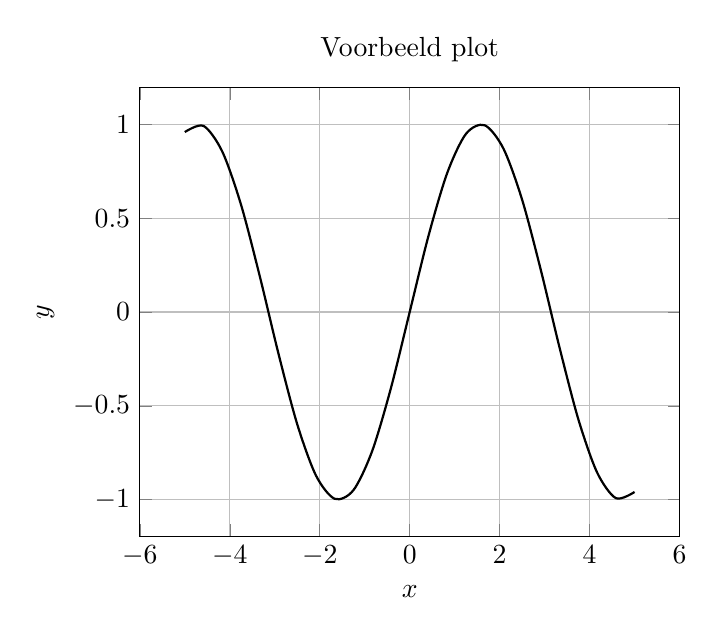
\begin{tikzpicture}
  \begin{axis}[title={Voorbeeld plot},xlabel={$x$},ylabel={$y$},grid=major]
    \addplot[smooth,thick] {sin(deg(x))};
  \end{axis}
\end{tikzpicture}

\subsection*{PGFPlots: meerdere subplots (groupplots)}
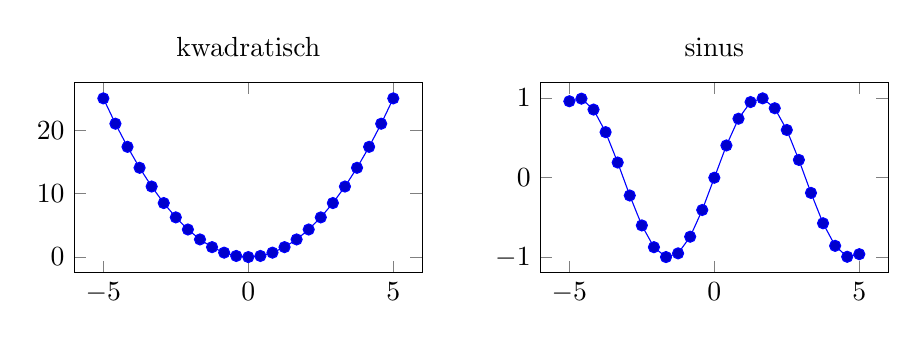
\begin{tikzpicture}
  \begin{groupplot}[group style={group size=2 by 1,horizontal sep=1.5cm},height=4cm,width=6cm]
    \nextgroupplot[title={kwadratisch}]
      \addplot {x^2};
    \nextgroupplot[title={sinus}]
      \addplot {sin(deg(x))};
  \end{groupplot}
\end{tikzpicture}

\subsection*{tcolorbox: theorema-box}
\begin{tcolorbox}[colback=blue!5,colframe=blue!40,title=Stelling]
  \textbf{Stelling.} Als $f$ continu is op $[a,b]$ dan heeft $f$ een maximum en minimum op $[a,b]$.
\end{tcolorbox}

\subsection*{Code listings (listings)}
\begin{lstlisting}[language=Python,caption={Voorbeeld Python code},label={lst:py1}]
def mean(xs):
    return sum(xs)/len(xs)
\end{lstlisting}

% Optional: minted (requires \texttt{--shell-escape})
% \begin{minted}[fontsize=\small]{python}
% def mean(xs):
%     return sum(xs)/len(xs)
% \end{minted}

\subsection*{Glossaries (definities)}
\IfFileExists{glossaries.sty}{%
  \noindent Voorbeeld: \gls{Ra} (gebruik \verb|glossaries| om een glossarium te maken).
}{%
  \noindent Voorbeeld: Ra (installeer het pakket \texttt{glossaries} om een glossarium te gebruiken).
}

\subsection*{Bibliografie (biblatex)}
\IfFileExists{biblatex.sty}{%
  Aanhaling voorbeeld: \parencite{Lamport1994}.
  \printbibliography[heading=subbibliography]
}{%
  \noindent Bibliografie voorbeeld vereist \texttt{biblatex} (installeer via \texttt{tlmgr install biblatex}).
}

\subsection*{Cheat‑sheet stijl (multicol)}
\IfFileExists{multicol.sty}{%
  \begin{multicols}{2}
    \begin{itemize}
      \item Kort item 1
      \item Kort item 2
      \item Kort item 3
    \end{itemize}
  \end{multicols}
}{%
  % multicol niet beschikbaar
}

\subsection*{Wiskunde: Aligned Equations}
Gebruik de \texttt{align*} omgeving voor het uitlijnen van berekeningen:
\begin{align*}
  F_c &= k_c \cdot a \cdot f \\
      &= \num{2500} \cdot \num{2.5} \cdot \num{0.2} \\
      &= \SI{1250}{\newton}
\end{align*}

\subsection*{Chemische notatie (mhchem)}
Gebruik \verb|\ce{...}| voor chemische formules: \ce{H2O}, \ce{Fe2O3}, of reacties:
\begin{center}
  \ce{2H2 + O2 -> 2H2O}
\end{center}

\subsection*{Hyperlinks}
\begin{itemize}
  \item Klikbare URL: \url{https://www.latex-project.org/}
  \item Link met tekst: \href{https://en.wikibooks.org/wiki/LaTeX}{LaTeX Wikibook}
\end{itemize}

\subsection*{TikZ: Flowchart (Productieproces)}
\begin{center}
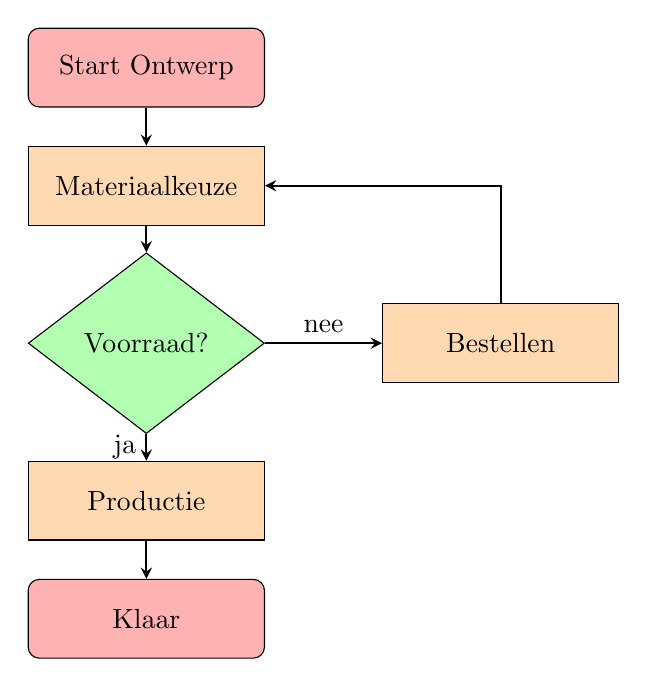
\begin{tikzpicture}[
    node distance=1.5cm,
    startstop/.style={rectangle, rounded corners, minimum width=3cm, minimum height=1cm,text centered, draw=black, fill=red!30},
    process/.style={rectangle, minimum width=3cm, minimum height=1cm, text centered, draw=black, fill=orange!30},
    decision/.style={diamond, minimum width=3cm, minimum height=1cm, text centered, draw=black, fill=green!30},
    arrow/.style={thick,->,>=stealth}
]
    \node (start) [startstop] {Start Ontwerp};
    \node (pro1) [process, below of=start] {Materiaalkeuze};
    \node (dec1) [decision, below of=pro1, yshift=-0.5cm] {Voorraad?};
    \node (pro2a) [process, below of=dec1, yshift=-0.5cm] {Productie};
    \node (pro2b) [process, right of=dec1, xshift=3cm] {Bestellen};
    \node (stop) [startstop, below of=pro2a] {Klaar};

    \draw [arrow] (start) -- (pro1);
    \draw [arrow] (pro1) -- (dec1);
    \draw [arrow] (dec1) -- node[anchor=east] {ja} (pro2a);
    \draw [arrow] (dec1) -- node[anchor=south] {nee} (pro2b);
    \draw [arrow] (pro2b) |- (pro1);
    \draw [arrow] (pro2a) -- (stop);
\end{tikzpicture}
\end{center}

\vspace{1em}
\noindent --- Einde template ---
\end{document}